\section{Presentations? - Custom Beamer Template}
    \begin{frame}{Beamer: LaTeX way of writing Presentations}
        \begin{itemize}
            \item Write presentations like your papers/thesis in \LaTeX \pause
            \item Reuse formulas/images/code/sources \pause
            \item Consistent style \& references    \pause
            \item Version control    \pause
            \item Easier collaboration
        \end{itemize}

        \blankfootnote{Beamer \cite{beamerPackageCtan} \tab{} Template \cite{selfBeamerTemplateMNTF}}
    \end{frame}

    \note[enumerate]{
        \item Re-use tooling, editor, setup (even this on overleaf alone much better that shared powerpoint presentation)
        \item This presentation, report and thesis all live in one git-repository and share resources
        \item Everything I ever work on is hosted in Git.
        \begin{itemize}
            \item Without Version Control it is no longer possible for me to work effectively
            \item Every workflow is massively ensured by it
            \item Also for single-person work, but built in collaboration, synchronization and backup
        \end{itemize}
    }

    \begin{frame}{Minimal example for beamer presentation}
        \begin{columns}
            \column{0.4\textwidth}
                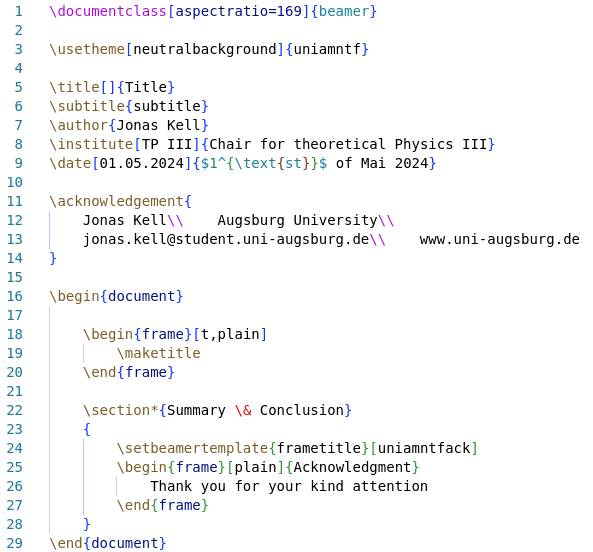
\includegraphics[width=1.1\textwidth]{./beamer-minimal-example/code.png}
            \column{0.4\textwidth}
                
\includegraphics[width=0.9\textwidth]{./beamer-minimal-example/result.png}
        \end{columns}
    \end{frame}

    \note[enumerate]{
        \item 29 lines gets you a basic presentation
        \item First time very much slower as putting together by hand in PowerPoint
        \item If you want to do crazy stuff, possible but really hard
        \item Actually quite a timesaver when you have an example/template to work of and do not require crazy levels of features
        \item When it works, perfectly portable (just a pdf), high performant and versatile (output rendering of presentation, notes, animations from one source)
        \item If proper presentation tools, has all the bells and whistles (presentation timer, pointer, multi-view presentation and more)
    }
